\documentclass[beamer]{standalone}
\begin{document}

\title[Electronics]{Resistors and simple network analysis}

\begin{frame} 
  \titlepage
\end{frame}

% Structuring a talk is a difficult task and the following structure
% may not be suitable. Here are some rules that apply for this
% solution: 

% - Exactly two or three sections (other than the summary).
% - At *most* three subsections per section.
% - Talk about 30s to 2min per frame. So there should be between about
%   15 and 30 frames, all told.

% - A conference audience is likely to know very little of what you
%   are going to talk about. So *simplify*!
% - In a 20min talk, getting the main ideas across is hard
%   enough. Leave out details, even if it means being less precise than
%   you think necessary.
% - If you omit details that are vital to the proof/implementation,
%   just say so once. Everybody will be happy with that.

\begin{frame}{Welcome to Electronics}
 \begin{itemize}
  \item Compression\ldots
  \item Photo and introductions
  \begin{itemize}
   \item Your name, class, major
   \item What is your previous experience with electronics?
   \item What are your expectations for this course?
   \item What is your favorite food? % no right or wrong answer
  \end{itemize}
 \end{itemize}
\end{frame}

\section{Syllabus}
\begin{frame}
\frametitle{Analog Electronics goals}
 Major time spending for experiment preparation goes to design,
 construction and interfacing  different electronics components.
 
 Often a commercial circuitry is not available or it has to be matched
 with electronics front-ends (responsible for collecting usually weak
 signals)  or back-ends (which do general purpose processing).

 To perform above tasks we need:
 \begin{itemize}
  \item Learn basic discrete components
  \begin{itemize}
   \item resistors, capacitors, inductors.
   \item diodes, photo-diodes, transistors, FETs.
   \item op-amps, comparators.
  \end{itemize}
  \item Multimeters, oscilloscopes, function generators.
  \item Breadboards and soldering irons.
  \item Modern circuit design and lay-out software.
  \item Master their usage.
 \end{itemize}
 As result you will be capable to build simple yet capable electronics circuits.
\end{frame}

\begin{frame}
\frametitle{From schematic to the board layout}
 \begin{columns}[c]
  \begin{column}{.18\textwidth}
   Schematic
  \end{column}
  \begin{column}{.82\textwidth}
    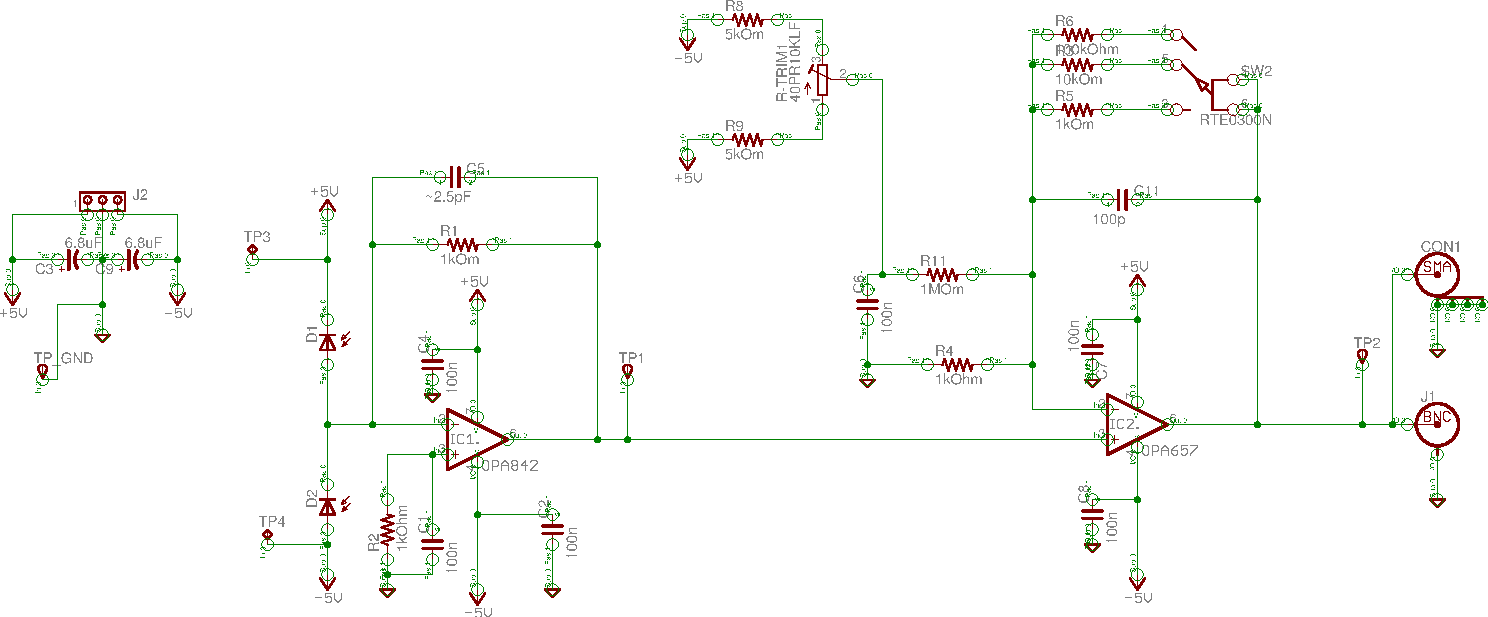
\includegraphics[width=0.9\textwidth]{./pics/bpd_v3_schematics.pdf}
  \end{column}
 \end{columns}

 \vskip .2in
 \begin{columns}[t]
  \begin{column}{.5\textwidth}
   Board layout
   \begin{figure}
   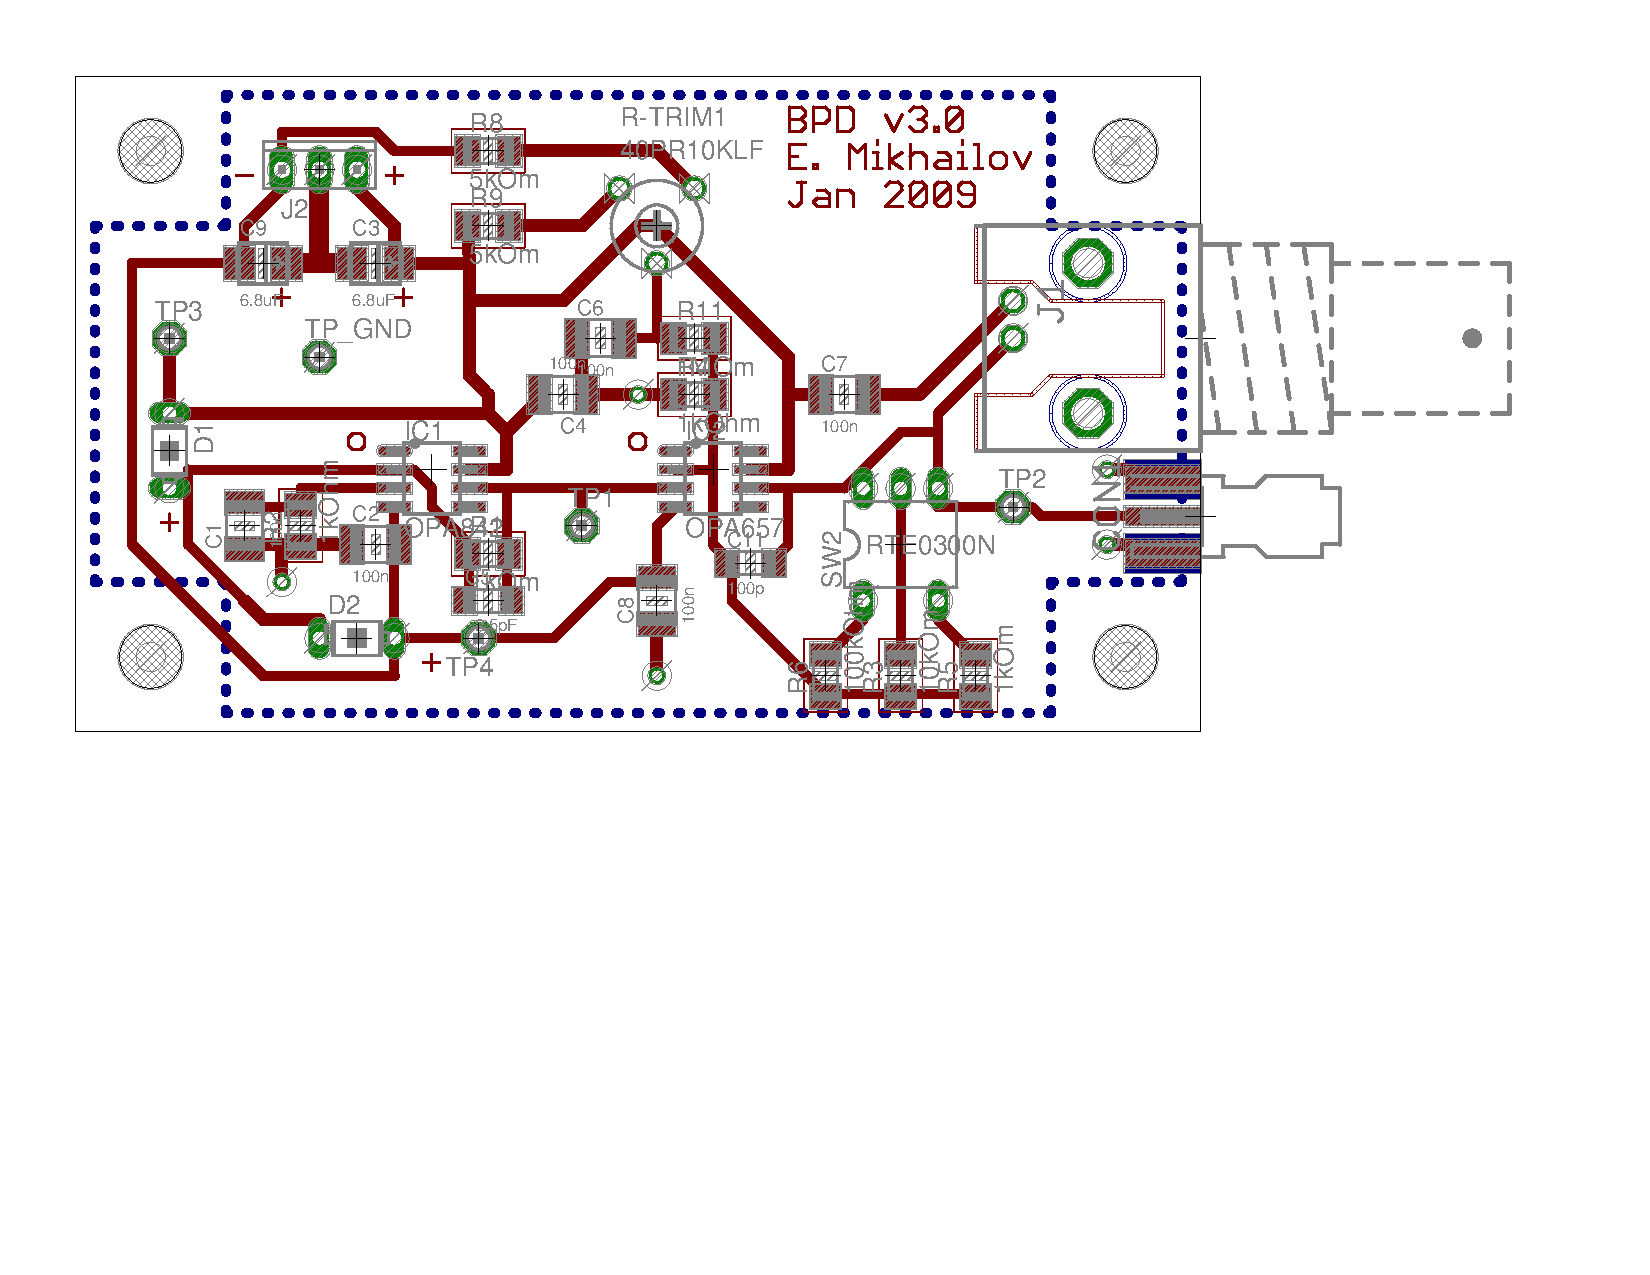
\includegraphics[angle=0,width=0.99\textwidth]{./pics/bpd_v3_board.pdf}
   \end{figure}
  \end{column}
  \begin{column}{.5\textwidth}
   Hardware
   \begin{figure}
   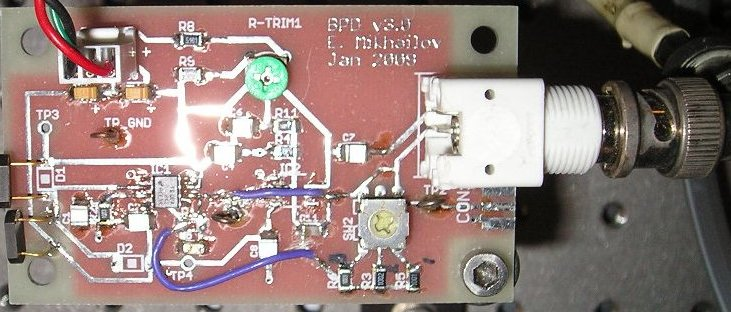
\includegraphics[angle=0,width=0.99\textwidth]{./pics/PDboard_finished}
   \end{figure}
  \end{column}
 \end{columns}
\end{frame}


\begin{frame}
\frametitle{Contact info}
{\bf Instructor: Wouter Deconinck}
\begin{itemize}
 \item Office: Small Hall 343D
 \item Lab: Small Hall 234
 \item Phone: 221-3539 (office)
 \item Email: \htmladdnormallink{wdeconinck@wm.edu}{mailto:wdeconinck@wm.edu}
 \item Office Hours: by appointment through \url{http://doodle.com/wdeconinck}.
\end{itemize}

{\bf T.A. lab book graders: Charlie Fancher, Drew Rotunno}

\end{frame}

\begin{frame}
\frametitle{Evaluations}
Your final grade for the course will be determined from the following grading weight distribution:

\begin{itemize}
\item Lab Book:   35\%
\item Design Exercises:  10\%
\item Quizzes:  5\%
\item Participation:  10\%  (\alert{being in class/lab is not enough})
\item Midterm:   20\%
\item Final:   20\%
\end{itemize}
\end{frame}


\begin{frame}
\frametitle{Lab books}
Your lab book is \alert{the primary record of your work and data}.  

\begin{itemize}
 \item What you did.
 \item How you did it (e.g. circuit diagrams).
 \item How you made measurements (which test equipment and how it was connected).
 \item Your data and enough information to tell us what that data is.
 \item What you observed (oscilloscope traces).
 \item Your calculations and analysis (including scratch work). 
 \item Plots (labeled axes).
 \item Answers to questions and justifications for your answers.
\end{itemize}

Once something is entered in your lab book it should never be modified, only amended by making a clear comment or by referring to a later page.
\end{frame}


\begin{frame}
\frametitle{Lab books}

\begin{block}{Neatness of Your Lab Books}
Diagrams, data, graphs, and other notes on separate pieces of paper should be
glued, taped, or stapled into the lab book.

\alert{If something falls out of the lab book during reading, shaking, transporting,
it is not the part of the lab book and will be discarded.}

The lab book will be graded primarily on completeness but to some extent also on neatness.
It should be clear and readable for the grader and yourself!
\end{block}

\begin{block}{Design Exercises}
Most labs will include a design exercise.
\alert{The designs must be prepared in your lab book prior to attending a lab}.
I will check preparation of the design exercise at the beginning of each lab.
\alert{An unprepared/incomplete design exercise will have at least 50\% penalty.}
\end{block}
\end{frame}


\begin{frame}
\frametitle{Due days}
\begin{block}{Lab Books}
Lab books are due by 9:00 pm on the next day after lab (i.e. Wednesday for the Tuesday section, Thursdays for the Wednesday section, and Fridays for the Thursday section) and will be returned by the next lab period.

Late lab books submission will have  points deducted. If you  know you will have a problem getting  the report on time please send me  an email as soon as you can to let me know about your situation.
\end{block}

\begin{block}{Illness}
Please notify the instructor if you are ill, so that arrangements can be made to make up missed labs.
\end{block}
\end{frame}


\begin{frame}
\frametitle{Tests and Exams}
\begin{block}{Pre-Lecture Quizzes}
Pre-lecture quizzes are \textbf{due by 10am} on the day of the lecture (on blackboard).  They will test that you have engaged with the readings, and will not include any difficult problems.
\end{block}

\begin{block}{Midterm exam}
There will a 1 hour midterm exam in lab the \textbf{week of March 2} (before spring break). There will be a shortened lab session after the midterm.
\end{block}

\begin{block}{Final exam}
There will be a final exam on \textbf{Monday May 4, 9:00 am--noon} (to be confirmed) covering all course materials.
\end{block}
\end{frame}


\begin{frame}
\frametitle{Grades table}
\begin{center}\begin{tabular}{|l|l|l|l|l|l|}
\hline \textbf{Grade} & \textbf{Score} & \textbf{Grade} &
\textbf{Score} & \textbf{Grade} & \textbf{Score} \\
\hline A- & 90-93 & A & 93-100 &    &       \\
\hline B- & 80-83 & B & 83-86  & B+ & 86-90 \\
\hline C- & 70-73 & C & 73-76  & C+ & 76-80 \\
\hline D- & 60-63 & D & 63-66  & D+ & 66-70 \\
\hline F  & $<$60 &   &        &    &       \\
\hline \end{tabular}\end{center}
\end{frame}


\begin{frame}
\frametitle{Calendar}
\url{http://blackboard.wm.edu}
\end{frame}

\section{DC Circuits Basics}
\begin{frame}
 \frametitle{Basic blocks}
 \begin{block} { Voltage (V)}
  Short for electrical potential difference\\
  Potential energy divided by charge ($V=E/Q$) \\
  Derived Unit: J/C \\  
  SI unit: V (Volt)
 \end{block}
 
 \begin{block} { Current (I)}
  Rate of flow of electric charge ($dQ/dt$)\\
  SI unit: A (Ampere)
 \end{block}

 \begin{block} {Power (P)}
  Energy per time (dE/dt) \\
  In electronics: $P=V I$ \\
  SI unit: W (Watt)
 \end{block}
\end{frame}

\begin{frame}
 \frametitle{Electrical resistance}
 \begin{block} { Resistance (R) }
 Different objects have different current passing through when the same voltage difference is applied.
 
 Which indicates: they have different
 electrical resistance.

 SI unit: $\Omega$ (Ohm)
 \end{block}

 \begin{block}{Ohm's law}
 \[I = \frac{V}{R} \]
 \end{block}
\end{frame}

\begin{frame}
 \frametitle{Resistors}
 \begin{columns}[t]
  \begin{column}{.3\textwidth}
   Standard leaded
   \begin{figure}
   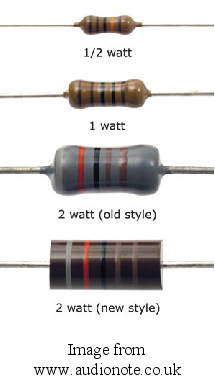
\includegraphics[width=0.85\textwidth]{./pics/resistors1.png}
   \end{figure}
  \end{column}
  \begin{column}{.3\textwidth}
   Power
   \begin{figure}
   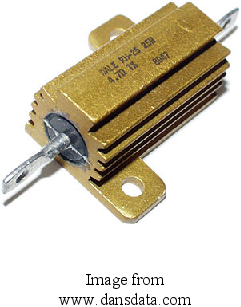
\includegraphics[width=0.85\textwidth]{./pics/resistors2.png}
   \end{figure}
  \end{column}
  \begin{column}{.3\textwidth}
   Surface mounted
   \begin{figure}
   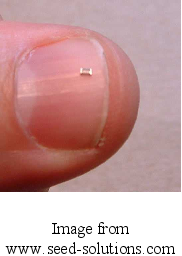
\includegraphics[width=0.85\textwidth]{./pics/resistors3.png}
   \end{figure}
  \end{column}
 \end{columns}
\end{frame}


\begin{frame}
 \frametitle{Resistor color code}
 \vskip -.1in
 \begin{figure}
  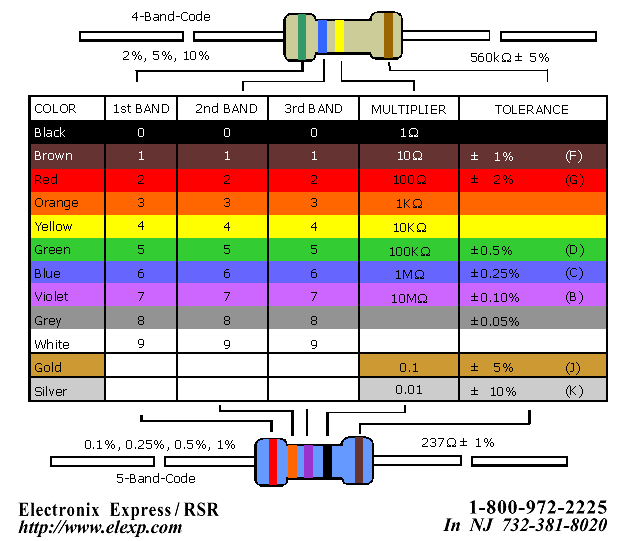
\includegraphics[width=0.8\textwidth]{./pics/clr_code.png}
 \end{figure}
\end{frame}

\begin{frame}
 \frametitle{Resistors usage} 
 \begin{itemize}
  \item current limiters
  \item fix voltage from a current source (exotic use)
  \item generate heat 
  \item fuse (non standard use)
  \item lowering the voltage of the source (i.e. voltage dividers)
 \end{itemize}
\end{frame}


\begin{frame}
 \frametitle{Combinations of resistors}
 \begin{block}{Series}
  \begin{equation*}
   R_{eq} = R_1 + R_2
  \end{equation*}
  \begin{itemize}
   \item Always $R_{eq} > R_1, R_2$
   \item If $R_1 \ll R_2$, then $R_{eq} \sim R_2$
  \end{itemize}
 \end{block}
 \begin{block}{Parallel}
  \begin{equation*}
   \frac{1}{R_{eq}} = \frac{1}{R_1} + \frac{1}{R_2} \quad \hbox{or} \quad R_{eq} = \frac{R_1 R_2}{R_1 + R_2}
  \end{equation*}
  \begin{itemize}
   \item Always $R_{eq} < R_1, R_2$
   \item If $R_1 \ll R_2$, then $R_{eq} \sim R_1$
  \end{itemize}
 \end{block}
\end{frame}


\section{Voltage divider}
\begin{frame}
 \frametitle{Unloaded voltage divider}
 \begin{columns}[c]
  \begin{column}{.3\textwidth}
   \begin{figure}
    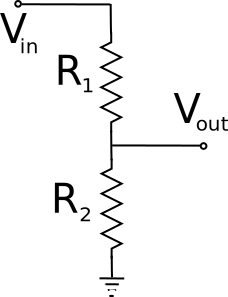
\includegraphics[height=2in]{./pics/unloaded_voltage_divider}
   \end{figure}
  \end{column}
  \begin{column}{.7\textwidth}
   \[ V_{out} = V_{in} \frac{R_2}{R_1+R_2} \]
  \end{column}
 \end{columns}
\end{frame}

\begin{frame}
 \frametitle{Loaded voltage divider}
 \begin{columns}[c]
  \begin{column}{.3\textwidth}
   \begin{figure}
    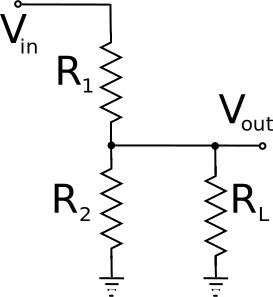
\includegraphics[height=2in]{./pics/loaded_voltage_divider}
   \end{figure}
  \end{column}
  \begin{column}{.7\textwidth}
   \[ V_{out,loaded} = V_{in} \frac{R_2}{R_1+R_2} \frac{R_L}{R_L + R_{1||2}} \]
   \[ V_{out,loaded} = V_{out,unloaded} \frac{R_L}{R_L + R_{1||2}} \]
  \end{column}
 \end{columns}
\end{frame}

\end{document}
